\section{mr::buffer\_\-base Struct Reference}
\label{structmr_1_1buffer__base}\index{mr::buffer_base@{mr::buffer\_\-base}}
{\tt \#include $<$mr\-Stream.h$>$}

Inheritance diagram for mr::buffer\_\-base::\begin{figure}[H]
\begin{center}
\leavevmode
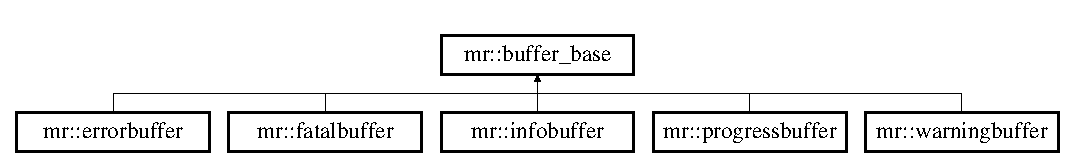
\includegraphics[height=1.80645cm]{structmr_1_1buffer__base}
\end{center}
\end{figure}
\subsection*{Public Member Functions}
\begin{CompactItemize}
\item 
{\bf buffer\_\-base} ()
\item 
virtual {\bf $\sim$buffer\_\-base} ()
\item 
virtual int {\bf sync} ()
\begin{CompactList}\small\item\em from basic\_\-streambuf, stl function used to sync stream \item\end{CompactList}\item 
virtual void {\bf print} (const char $\ast$const s)=0
\begin{CompactList}\small\item\em virtual function to print string out \item\end{CompactList}\end{CompactItemize}


\subsection{Constructor \& Destructor Documentation}
\index{mr::buffer_base@{mr::buffer\_\-base}!buffer_base@{buffer\_\-base}}
\index{buffer_base@{buffer\_\-base}!mr::buffer_base@{mr::buffer\_\-base}}
\subsubsection{\setlength{\rightskip}{0pt plus 5cm}mr::buffer\_\-base::buffer\_\-base ()\hspace{0.3cm}{\tt  [inline]}}\label{structmr_1_1buffer__base_a0}


\index{mr::buffer_base@{mr::buffer\_\-base}!~buffer_base@{$\sim$buffer\_\-base}}
\index{~buffer_base@{$\sim$buffer\_\-base}!mr::buffer_base@{mr::buffer\_\-base}}
\subsubsection{\setlength{\rightskip}{0pt plus 5cm}virtual mr::buffer\_\-base::$\sim${\bf buffer\_\-base} ()\hspace{0.3cm}{\tt  [inline, virtual]}}\label{structmr_1_1buffer__base_a1}




\subsection{Member Function Documentation}
\index{mr::buffer_base@{mr::buffer\_\-base}!print@{print}}
\index{print@{print}!mr::buffer_base@{mr::buffer\_\-base}}
\subsubsection{\setlength{\rightskip}{0pt plus 5cm}virtual void mr::buffer\_\-base::print (const char $\ast$const {\em s})\hspace{0.3cm}{\tt  [pure virtual]}}\label{structmr_1_1buffer__base_a3}


virtual function to print string out 



Implemented in {\bf mr::infobuffer} {\rm (p.\,\pageref{structmr_1_1infobuffer_a1})}, {\bf mr::warningbuffer} {\rm (p.\,\pageref{structmr_1_1warningbuffer_a1})}, {\bf mr::errorbuffer} {\rm (p.\,\pageref{structmr_1_1errorbuffer_a1})}, {\bf mr::fatalbuffer} {\rm (p.\,\pageref{structmr_1_1fatalbuffer_a1})}, and {\bf mr::progressbuffer} {\rm (p.\,\pageref{structmr_1_1progressbuffer_a1})}.\index{mr::buffer_base@{mr::buffer\_\-base}!sync@{sync}}
\index{sync@{sync}!mr::buffer_base@{mr::buffer\_\-base}}
\subsubsection{\setlength{\rightskip}{0pt plus 5cm}virtual int mr::buffer\_\-base::sync ()\hspace{0.3cm}{\tt  [virtual]}}\label{structmr_1_1buffer__base_a2}


from basic\_\-streambuf, stl function used to sync stream 



The documentation for this struct was generated from the following file:\begin{CompactItemize}
\item 
{\bf mr\-Stream.h}\end{CompactItemize}
